\section{Análise de Desempenho por Classe e Significância Estatística}

A análise detalhada da arquitetura campeã, a \textbf{DenseNet V10}, revela a robustez do modelo na distinção de classes comerciais de algodão. A Tabela \ref{tab:best_class_metrics} apresenta as métricas por categoria no conjunto de teste.

\begin{table}[!h]
    \centering
    \begin{threeparttable}
    \caption{Métricas detalhadas por classe para o modelo DenseNet V10.}
    \label{tab:best_class_metrics}
    \begin{tabular}{llll}
\toprule
 & Precisão & Revocação & Escore F1 \\
\midrule
31.2 & 0,628 & 0,744 & 0,681 \\
31.3 & 0,529 & 0,455 & 0,489 \\
31.4 & 0,492 & 0,547 & 0,518 \\
32.3 & 0,551 & 0,674 & 0,607 \\
32.4 & 0,778 & 0,406 & 0,533 \\
33.3 & 0,617 & 0,579 & 0,598 \\
41.4 & 0,619 & 0,441 & 0,515 \\
41.5 & 0,724 & 0,724 & 0,724 \\
42.4 & 0,673 & 0,434 & 0,528 \\
44.4 & 0,769 & 0,698 & 0,732 \\
\bottomrule
\end{tabular}

    \begin{tablenotes}
            \small 
            \item[] Fonte: Do autor.
        \end{tablenotes}
        \end{threeparttable}
\end{table}

A Matriz de Confusão Normalizada (Figura \ref{fig:matriz_v10}) corrobora estes achados, mostrando que a maioria dos erros ocorre entre classes adjacentes no espectro morfológico.

\begin{figure}[h!]
  \centering
  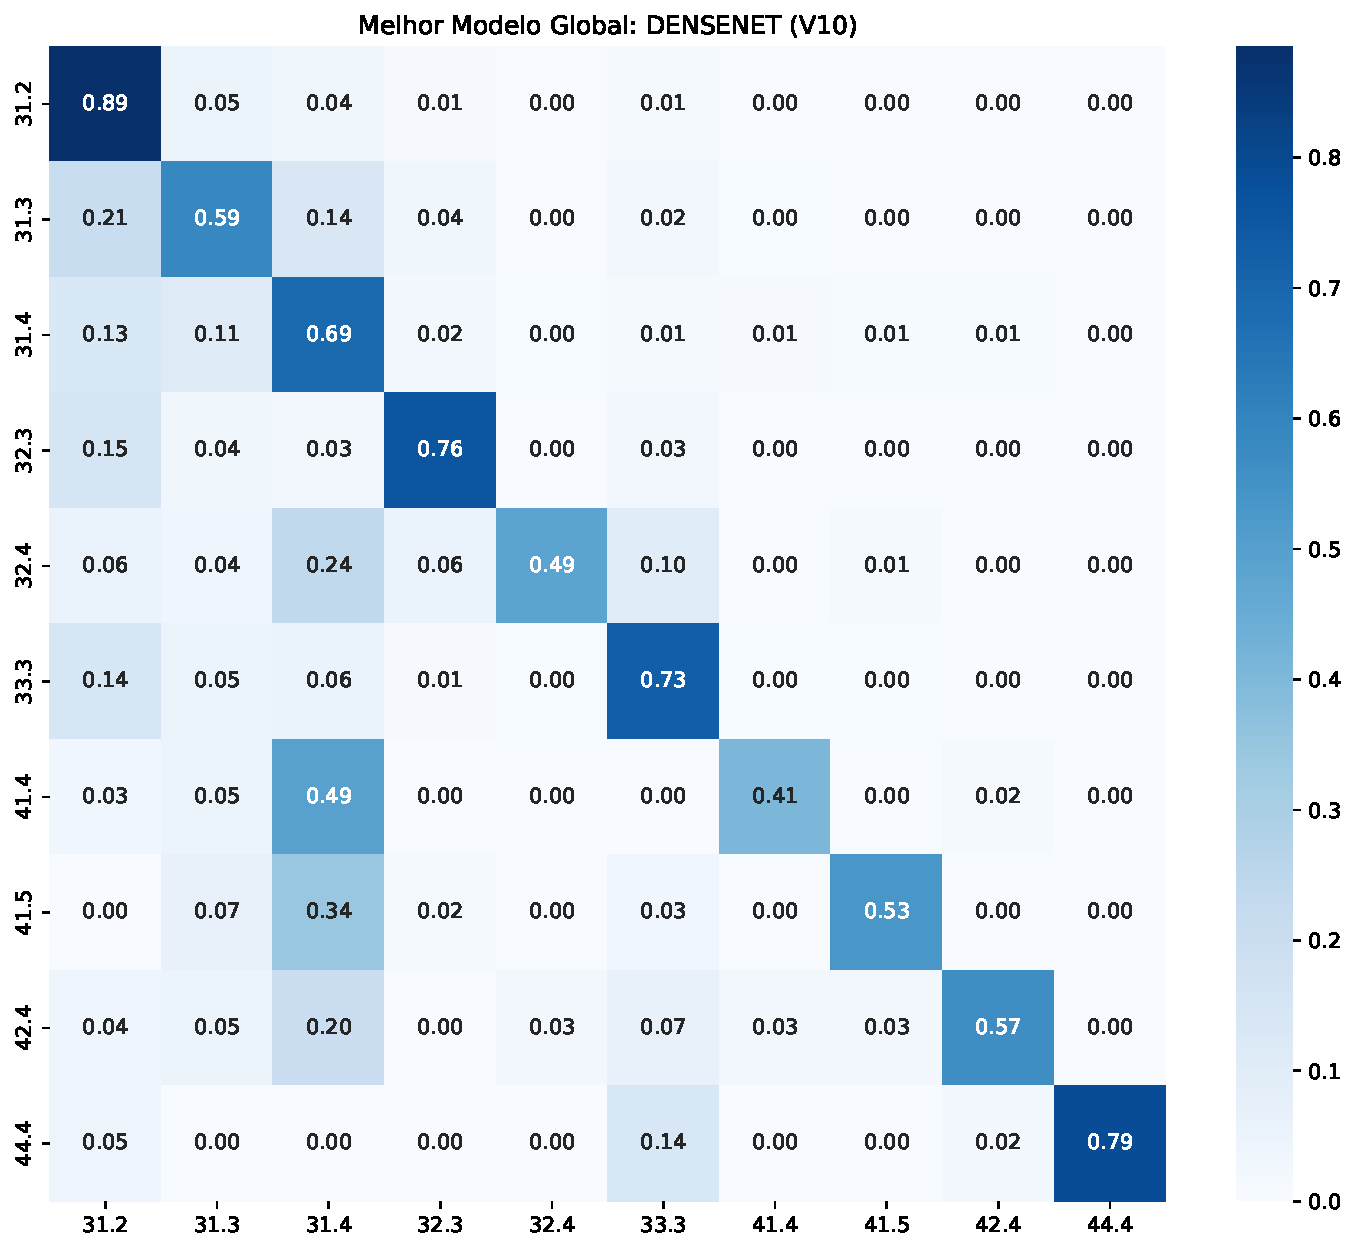
\includegraphics[width=0.9\textwidth]{images/best_model_confusion_matrix.pdf}
  \caption{Matriz de Confusão Normalizada para o modelo DenseNet V10.}
  \label{fig:matriz_v10}
\end{figure}

Para aprofundar a análise, a Figura \ref{fig:p_values_v10} apresenta a matriz de significância estatística (McNemar) entre os modelos. Um ponto crucial reside na comparação entre a \textbf{DenseNet} (líder em MCC) e a \textbf{ConvNext} (segunda colocada). O teste de McNemar revela que a superioridade da DenseNet sobre a ConvNext é estatisticamente significativa ($p < 0,05$). Isso indica que a DenseNet possui uma capacidade superior de capturar padrões discriminativos sutis que a ConvNext, apesar de sua arquitetura moderna, não consegue replicar integralmente neste conjunto de dados.

\begin{figure}[h!]
  \centering
  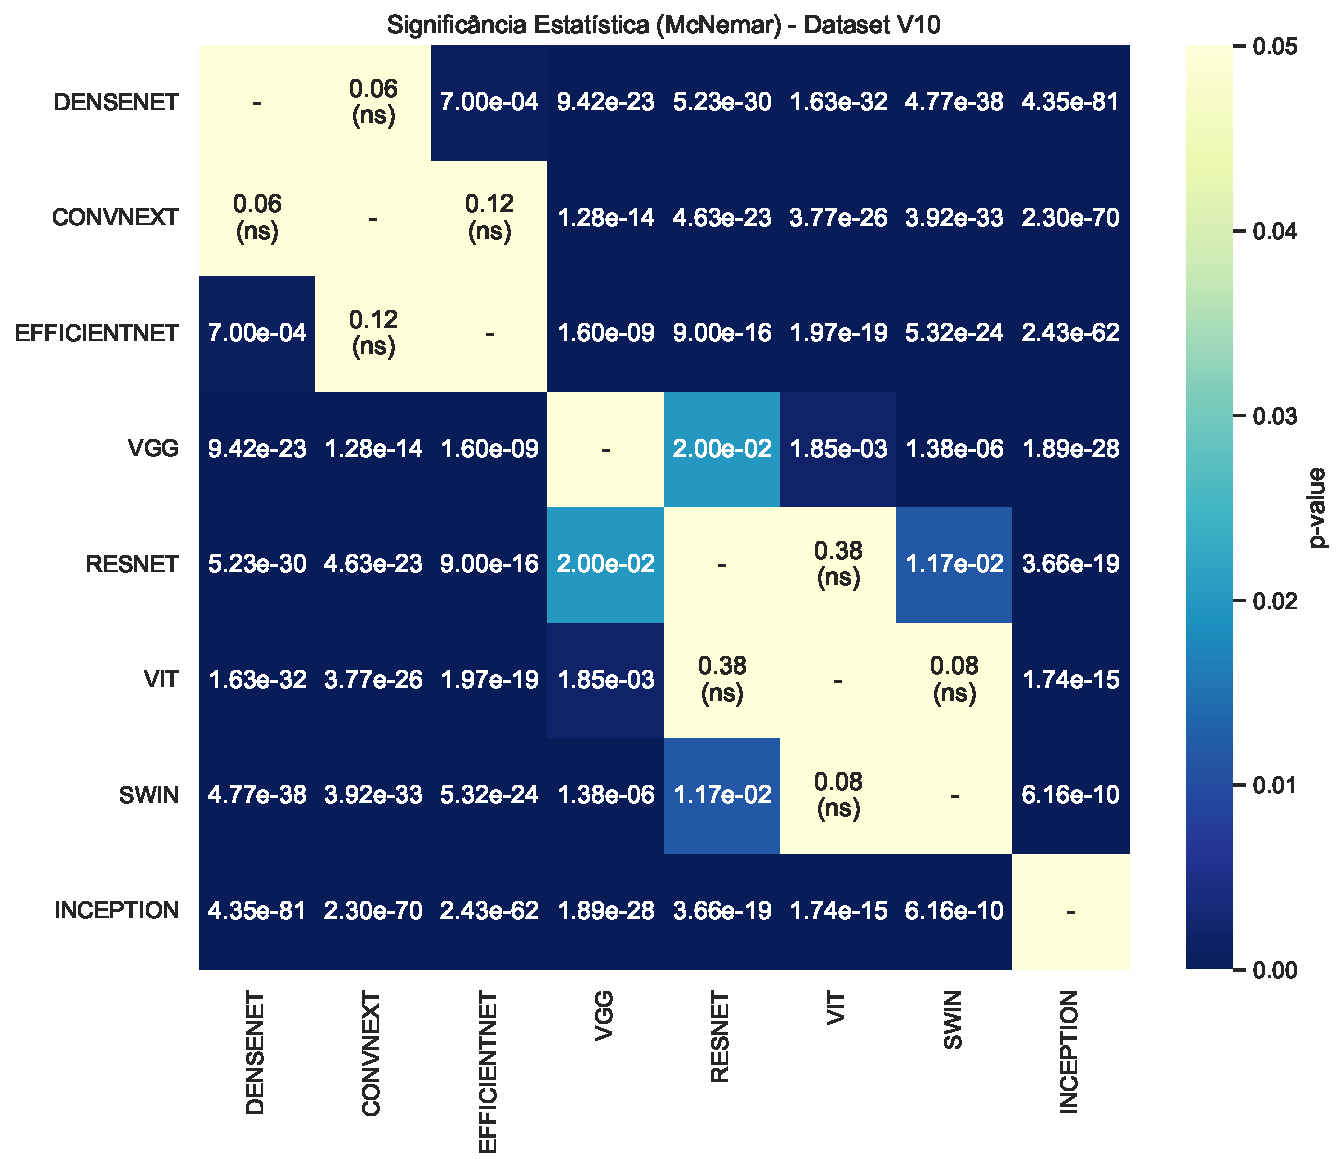
\includegraphics[width=0.8\textwidth]{images/p_value_heatmap_v10.pdf}
  \caption{Matriz de significância estatística (McNemar) no dataset V10. O sufixo (ns) indica ausência de diferença estatística.}
  \label{fig:p_values_v10}
\end{figure}
